\documentclass[11pt,a4paper]{article}
\usepackage[margin=2.5cm]{geometry}
\usepackage{amsmath,amssymb,booktabs,xcolor,enumitem,soul,graphicx,float}
\graphicspath{{../../../scripts/Images/}}
\usepackage[hidelinks]{hyperref}
\setlength{\parskip}{0.6em}\setlength{\parindent}{0pt}
\definecolor{newc}{HTML}{1f6f43}
\newcommand{\new}[1]{\textcolor{newc}{#1}}
\newcommand{\mockup}[1]{\textit{#1}}
\title{Proposed changes for [A91], agents that lock at a workstation}
\date{12 November 2026, version 2}
\begin{document}
\maketitle

\section*{How to read this}
Part~1 says what happens and what was decided, in plain words. Part~2 shows
the four places in the thesis that would change. Text in \new{green} is
proposed and not in the thesis yet. Black text is already there. Italic text
is a mockup instruction in the Experiments chapter. Part~3 lists the
questions for you. The rationale is entry [A91] in \texttt{GAPS.md}.

\section*{Part 1. What happens and what was decided}

\subsection*{The lock}
A workstation hangs off an aisle by a single edge. When that aisle is one
lane wide, the agents bringing lines to the workstation queue on it. The
agent at the workstation wants to step back onto the aisle, and the first
agent in the queue wants the workstation. That is a swap, so conflict
resolution makes both wait. The agents behind close the only way out, so the
wait lasts until an agent chooses to back out. The section around that
workstation stops. The rest of the fleet keeps working.

\subsection*{How often}
Over the 258 warehouse seeds of each fleet, a section whose four workstations
all hang off a one-lane aisle occurs in 35 seeds at 8 agents (14\,\%) and 70
seeds at 32 agents (27\,\%). Two of the six test seeds, 200000 and 200005,
have it at both fleet sizes.

Token Passing does not lock. It plans whole paths and keeps each vertex free
around every arrival, and every warehouse is well-formed. So the lock is a
limitation of the learned controllers on this family of layouts.

\subsection*{What was decided (11 November)}
\begin{itemize}[leftmargin=1.2em]
\item \textbf{No new rule.} A cap on open tasks per workstation was
discussed and dropped. It would change the assignment rule every controller
shares, and it fights the order model, where all lines of an order go to one
workstation. van Knippenberg et al.\ (2021) have no such rule either.
\item \textbf{No new layout.} Two-lane aisles would remove the lock, but
mean a new warehouse sweep with Token Passing.
\item \textbf{Train as it is.} Whether a controller learns to back out
becomes part of what is measured.
\item \textbf{Report it.} The number of locked test seeds per controller and
storage rule, a threat to validity, and under RQ4 whether messages make the
lock rarer.
\end{itemize}

\subsection*{What messages did so far}
One small test only, at 8 agents with congestion-aware storage, three test
seeds, checkpoint 8. With the rule for a locked seed you chose (Part~3), two
of the three seeds lock without messages and none with them. The fleet with
messages also finished more tasks (91 against 43, 155 against 107 and 201
against 143). Version~1 of this PDF said messages did not prevent the lock.
That used a looser test, one agent standing still for 50 steps, and is
corrected here. Three seeds are too few to claim more, so the full runs
decide.

\section*{Part 2. The text}

\subsection*{2.1 Implementation, ``When moves still clash''}
The new paragraph follows the one that ends with the circle of waiting
agents.

\begin{quote}
An agent is never ready when the agents it waits on form a circle, each
wanting the next one's vertex. A swap is the shortest such circle. These
agents wait, since none of them can move first.

\new{Such a circle can last. The clearest case is a workstation on an aisle
one lane wide. The agent at the workstation wants the aisle vertex in front
of it, and the agent queuing there wants the workstation. The agents queuing
behind close the only way out, so the wait ends only when an agent chooses
to back out. No rule is added to break it, because a rule would change the
assignment that every controller shares, and \textup{van Knippenberg et al.}
have none either. Whether the learned controllers learn to back out is part
of what is measured. Token Passing plans ahead and does not meet this
circle.}
\begin{figure}[H]
\centering
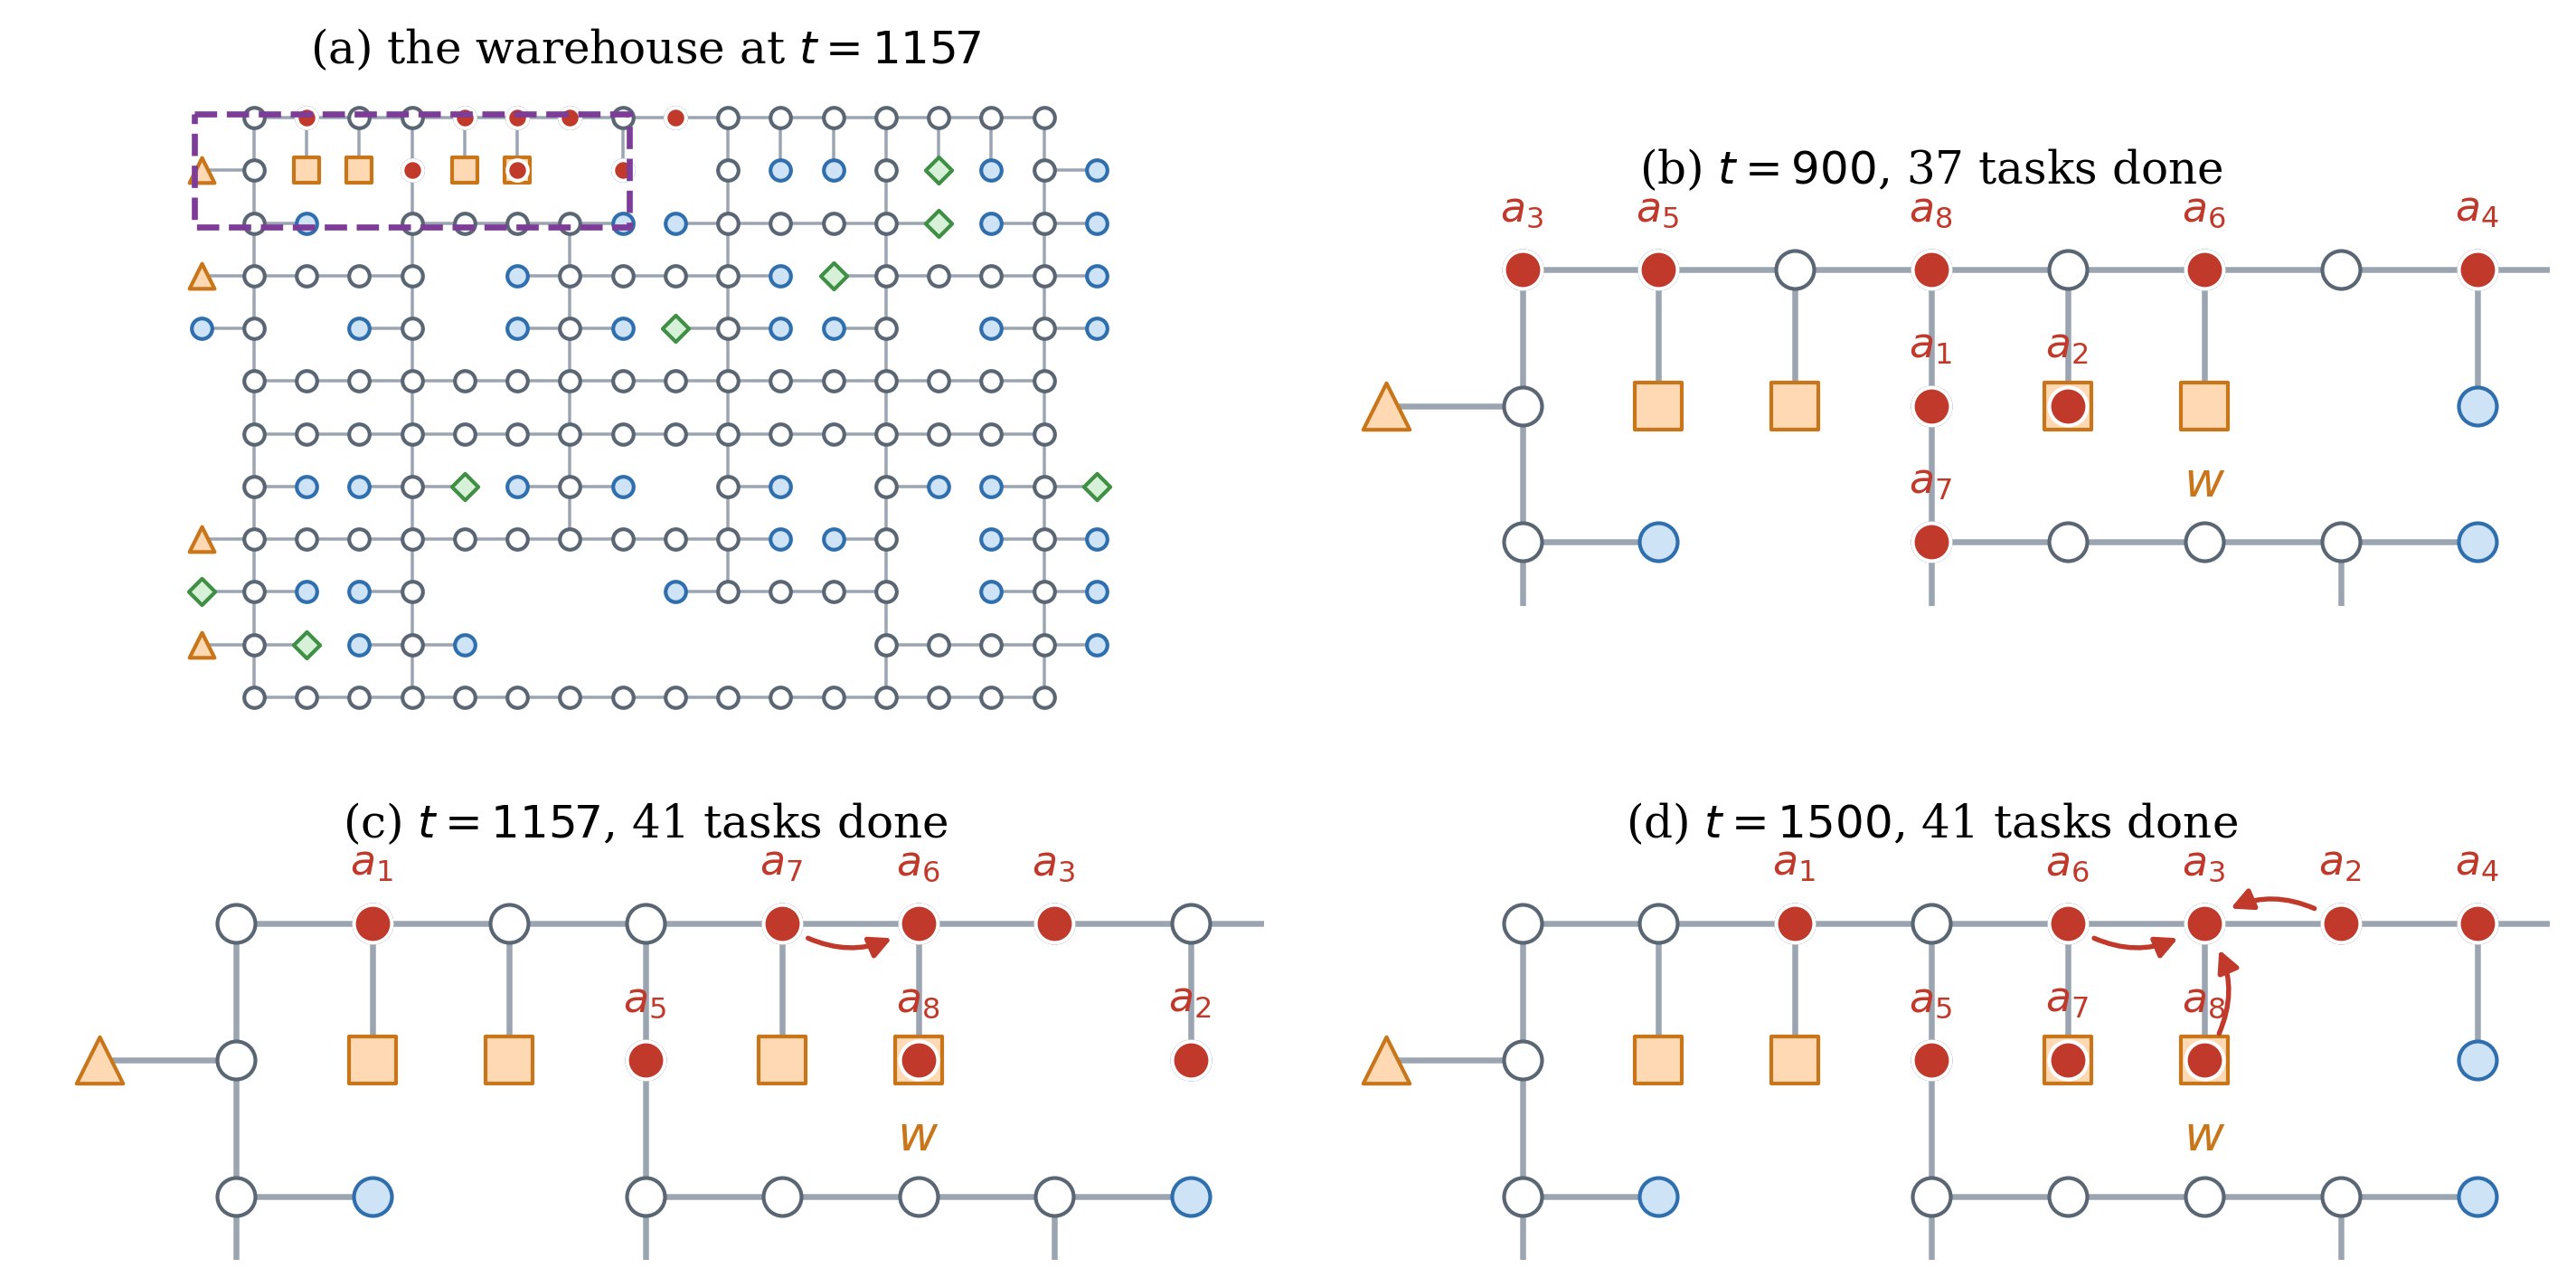
\includegraphics[width=\linewidth]{workstation_lock.png}
\caption{\new{A lock at workstation $w$ in test seed 200000 with eight
agents. Arrows show the move an agent asks for.}}
\label{fig:workstationlock}
\end{figure}

\new{Figure~\ref{fig:workstationlock} shows such a lock in a test warehouse
with eight agents. All four workstations of one section hang off the outer
aisle, which is one lane wide. At $t = 900$ the work still flows, and six
agents are on their way to the same workstation $w$. At $t = 1157$ agent $a_8$
has delivered at $w$ and must leave it for its next shelf. Agent $a_6$ stands
on the only vertex out and waits to enter $w$, and $a_7$ and $a_3$ queue
behind it. Neither $a_8$ nor $a_6$ can move first. Seven of the eight agents
are caught around this one workstation, so the whole fleet finishes only two
more tasks in the last 843 steps of the episode.}
\end{quote}

\subsection*{2.2 Experiments, Results, ``Keeping up''}
\begin{quote}
\textbf{Keeping up.} \mockup{Which conditions pass the keep-up check.
Report the backlog trace of one condition that falls behind, so the
reader sees what failing the check looks like.} \new{\mockup{Give the number
of test seeds that lock, per controller and storage rule. A seed locks when
at least two agents each hold the same task for 500 steps or more at the
same time, a quarter of the episode. A locked seed counts as not keeping
up.}}
\end{quote}

\subsection*{2.3 Experiments, Results, the communication paragraph}
\begin{quote}
\textbf{RQ5, communication (conditional).} \mockup{Only if reached. Gain of
the decentralised controller with messages over the same controller without.}
\new{\mockup{Also the number of locked test seeds with and without
messages.}}
\end{quote}
The paragraph still says RQ5. Since [A83] communication is RQ4. Renaming the
Results headings is a separate change and not part of this one.

\subsection*{2.4 Experiments, Discussion, ``Threats to validity''}
A new item in the list.
\begin{quote}
\begin{itemize}[leftmargin=1.2em]
\item \new{Agents can lock at a workstation on an aisle one lane wide
(Section~\textbackslash ref\{sec:method:resolution\}). A section with all its workstations on such aisles occurs in
14\,\% of the warehouses at 8 agents and 27\,\% at 32 agents, and in 5 of the
20 test warehouses at 8 agents. Token Passing
does not lock, so in these warehouses the gap between it and the learned
controllers is partly the layout.}
\end{itemize}
\end{quote}

\section*{Part 3. Decided, and what is left}
Your answers of 12 November.
\begin{enumerate}[leftmargin=1.4em]
\item \textbf{A seed is locked} when at least two agents each hold the same
task for 500 steps or more at the same time. The figure's seed locks from
$t = 1157$ by this rule.
\item \textbf{A locked seed counts as not keeping up.} Decided before the
evaluation, so the choice cannot follow the results.
\item \textbf{20 test seeds.} The runs already trained store 6 in their
settings, so the evaluation needs a small option in the code to play 20.
With 20 seeds, 5 have the layout at 8 agents (200000, 200005, 200012,
200017, 200018). The count for 32 agents is running.
\item \textbf{The mechanism goes in the Implementation chapter}, with the
figure, as in 2.1.
\end{enumerate}

Left for you. Is the figure's text right, and is the figure better beside
conflict resolution or beside the threats to validity? Every number here can
be made again with \texttt{thesis-progress/scripts/workstation\_lock.py}, and
\texttt{results/limitations/workstation\_lock/README.md} lists the commands.

\end{document}
